\documentclass[../../Aurora C# unofficial manual.tex]{subfiles}

\begin{document}
	\section{Adding moons and Lagrange points}\label{6_adding_moons_and_lagrange}
	Original post can be found
	\href{http://aurora2.pentarch.org/index.php?topic=8495.msg118787#msg118787}{here}.
	\\\\
	
	Below is the form for adding moons to existing planets. During planet creation you can specify appropriate moons to be created at the same time using standard moon generation based on the type of planet and is orbital distance. This form, accessed via the Add Moons button, is for creating additional moons which do not have to obey normal size restrictions. The form allows the addition of up to five moons (the drop-downs all start with no moon) with type and distance specified. If more than five moons are needed, the form can be used multiple times for the same parent planet.
	
	After initial generation you can use Modify Body to specify additional detail if required.
	
	The Add Lagrange button adds a Lagrange point to the currently selected body, even if it would not normally qualify for one.
	\begin{figure}[H]
		\centering
		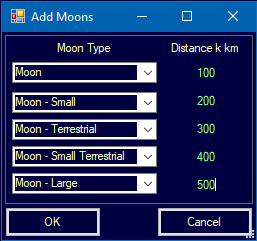
\includegraphics[width=0.5\linewidth]{images/AddMoons}
		\caption[Add Moons Example]{Add Moons Example}
		\label{fig:addmoons}
	\end{figure}
\end{document}